\section{Parameter Exploration}
A fast transition of the initial dominating end state to the desired dominating end state was observed by monitoring the dominating end state over time.
The transition occurred latest after $0.5$~ns, and the system remained in the biased end state for the rest of the simulation time.
In both water and complex simulations, the desired end state was sampled about $~99\%$ of the simulation time with the exception of L19 in water (Table \ref{SItab:RingCycleOpenin_sampling_fraction_optimizedStates}).
To inspect if the optimized state simulations' results sufficiently represent the target states, a comparison between the target state obtained potential energy distributions in the eds simulations with MD simulations consisting of only the target state was conducted (Figure \ref{fig:CHK1_set2_stateOptimization_EnergyDistribution}). 

\begin{table}[h]
\centering
\caption{Fraction of the simulation time (in \%) that the desired end state was sampled as the dominating state during the EDS simulation to optimize the coordinates for a desired end state.}
\label{SItab:RingCycleOpenin_sampling_fraction_optimizedStates}
\begin{tabular}{ l | c c }
 Ligand & Water  & Complex \\ 
 \hline
     L1 & 99.84 & 99.97 \\ 
     L17 & 99.99 & 99.97\\
     L19 & 36.07 &  99.98\\
     L20 & 99.99 & 100\\
     L21 & 100 & 99.97 \\
\end{tabular}
\end{table}

\begin{table}[h]
\centering
\caption{Potential thresholds for occurrence sampling ($T_{i}^{\text{phys}}$) and undersampling ($T_{i}^{\text{us}}$) determined during the parameter exploration (in kJ~mol$^{-1}$).}
\label{SItab:RingCycleOpenin_PotentialTresholds}
\begin{tabular}{ l | c c |c c| }
 Ligand &\multicolumn{2}{c|}{Water} & \multicolumn{2}{c|}{Complex}\\ 
  & \multicolumn{1}{c}{$T^{\text{phys}}$}& \multicolumn{1}{c|}{$T^{\text{us}}$}&  \multicolumn{1}{c}{$T^{\text{phys}}$}& \multicolumn{1}{c|}{$T^{\text{us}}$} \\ 
 \hline
     L1  & -582.96 & -436.05 & -737.37 & -516.41\\ 
     L17 & -572.41 & -419.16 & -717.95 & -492.83\\
     L19 & -579.13 & -415.91 & -738.95 & -483.78\\
     L20 & -636.00 & -492.75 & -759.01 & -549.35\\
     L21 & -656.22 & -488.43 & -805.30 & -539.78\\
\end{tabular}
\end{table}

\begin{figure}[h]
\centering
     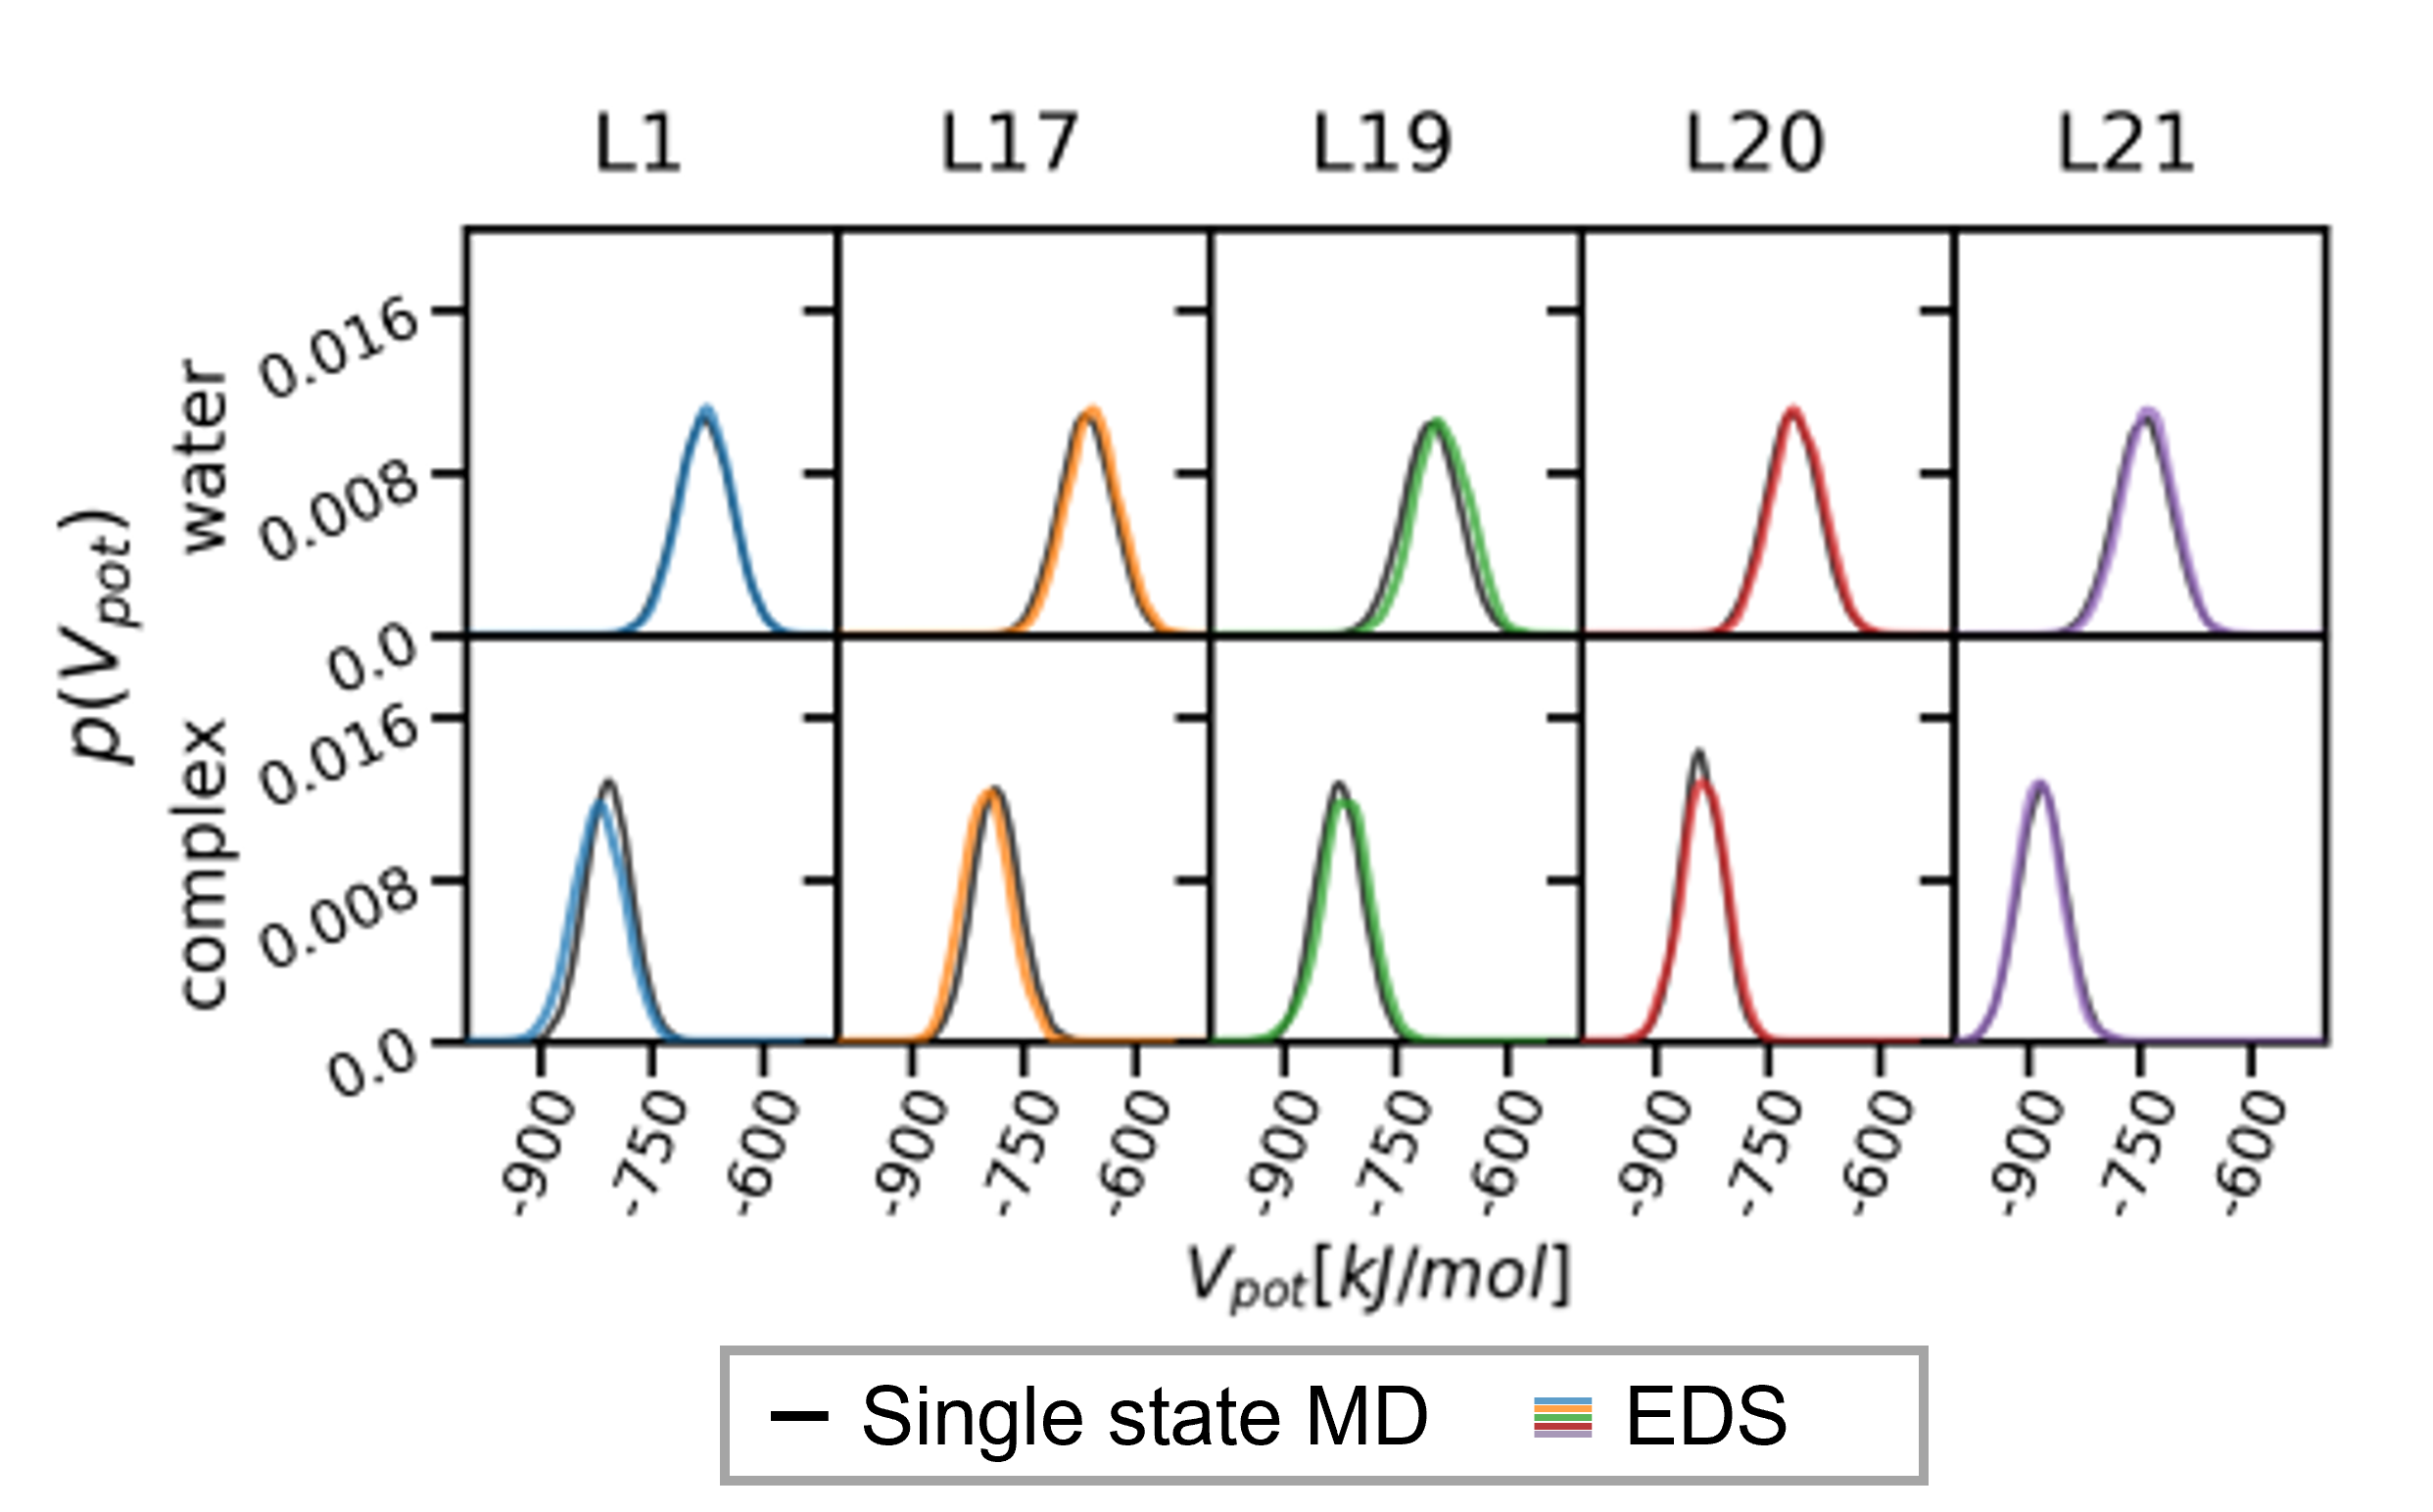
\includegraphics[width=0.8\textwidth]{fig/results/ringOpening/paramExploration/single_state_energy_sampling.png}
    \caption{Comparison of the potential-energy distribution obtained from a standard MD simulation of a given end state (black) and from an EDS simulation with the given end state favoured (colored) from the first step of the RE-EDS workflow.}
     \label{fig:CHK1_set2_stateOptimization_EnergyDistribution}
\end{figure}


\section{Energy Offset Estimation}
The relative energy offsets $\Delta \Delta E^R_{ji}$ are compared with the experimental relative binding free energies $\Delta \Delta G^\text{bind}_{ji}$ in Figure \ref{SIfig:Eoff_experiment_corr_RingOpening}. 
The root mean squared error (RMSE) between $\Delta \Delta E^R_{ji}$ obtained with RE-EDS 1SS and $\Delta \Delta G^\text{bind}_{ji}$ is $12.6$~kJ~mol$^{-1}$. Outliers are mainly related to L19.
With the RE-EDS SSM approach, the RMSE was reduced to $7.0$~kJ~mol$^{-1}$. No clear outliers were observed in this case. Thus, the use of the SSM approach is recommended for RE-EDS simulations.

The energy offsets obtained with the SSM approach are shown as a function of the replica ($s$-value) in Figure \ref{SIfig:Eoff-perreplica}. 

\begin{figure}[h]
\centering
  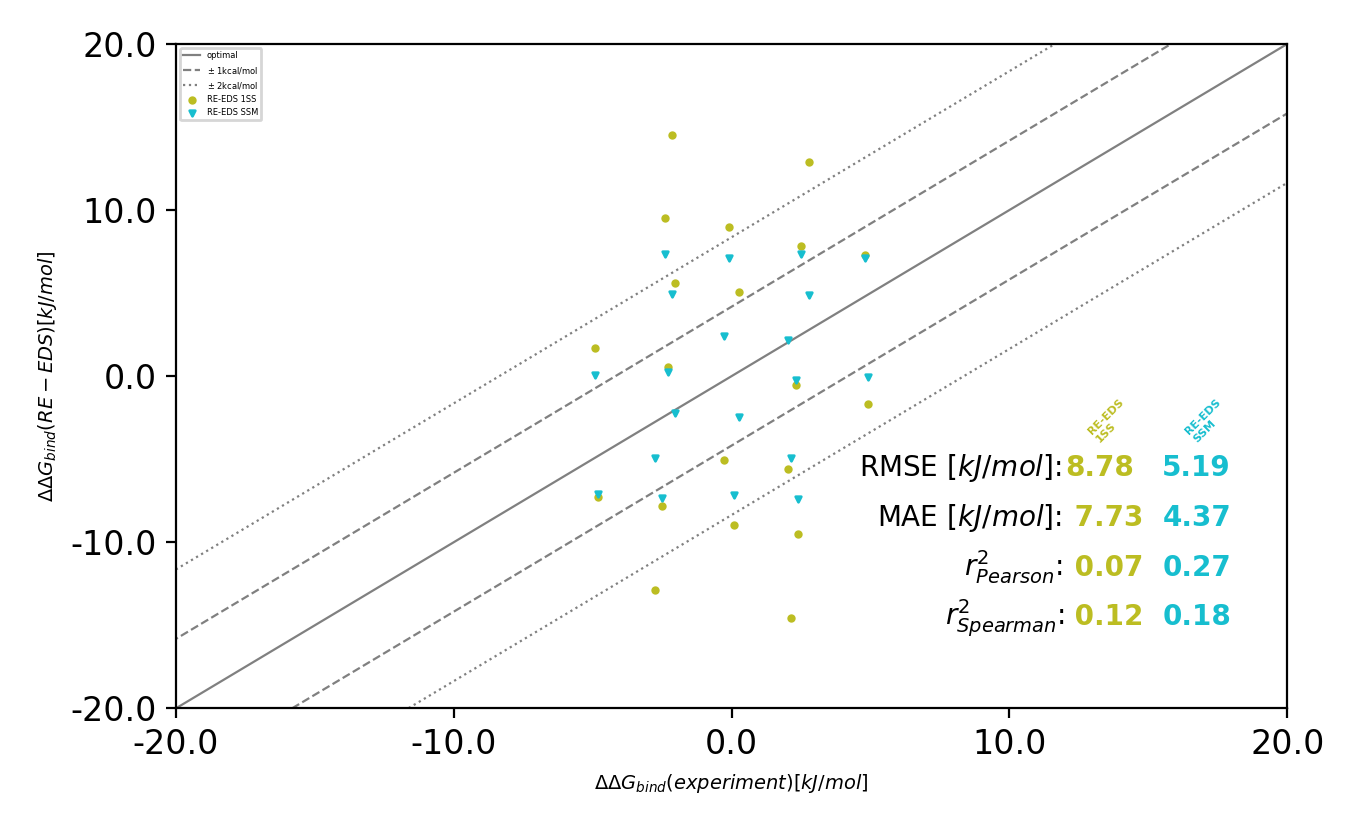
\includegraphics[width=0.8\textwidth]{fig/results/ringOpening/paramOptimization/RingClosure_system_Eoff_final_results.png}
\caption{Comparison of the relative energy offsets $\Delta \Delta E^R_{ji}$ in water and complex with the experimental relative binding free energies $\Delta \Delta G^\text{bind}_{ji}$. The energy offsets were estimated from RE-EDS simulations using the 1SS (green) or SSM (blue) approach to select the starting configurations of the replicas.} \label{SIfig:Eoff_experiment_corr_RingOpening}
\end{figure}

\begin{figure}[h]
\centering
  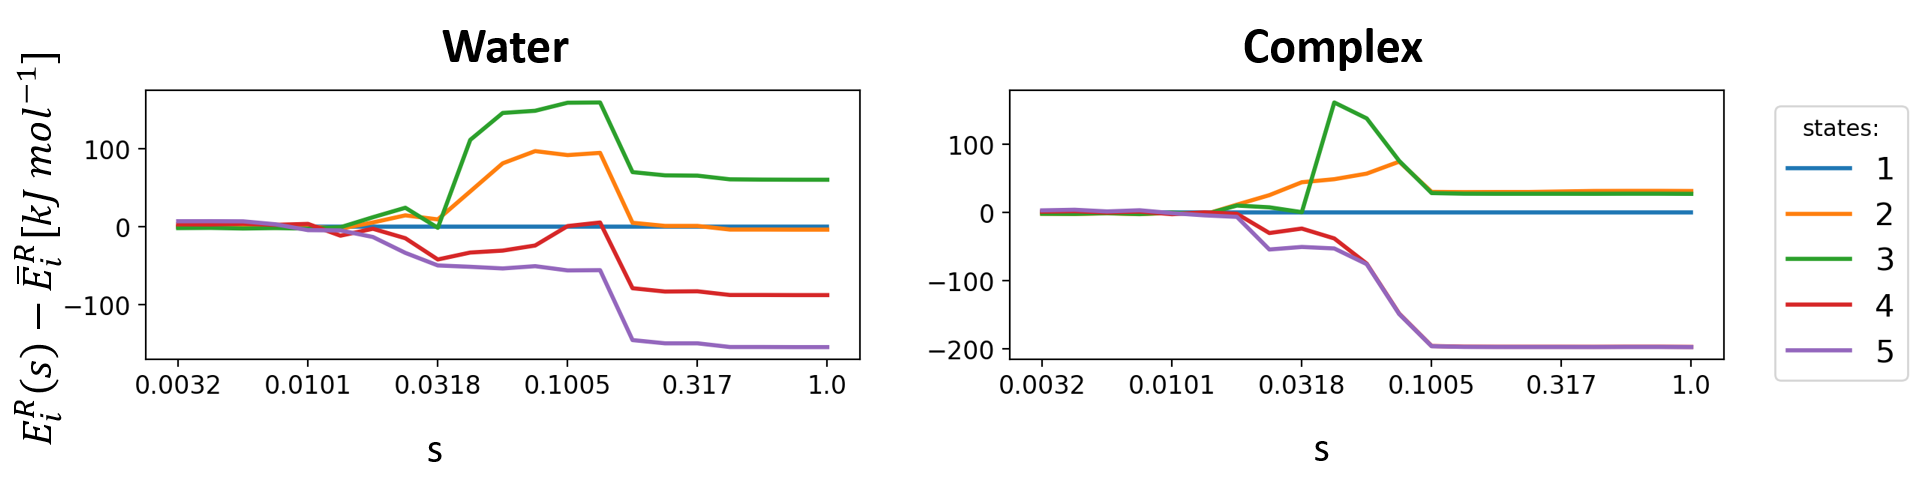
\includegraphics[width=1.0\textwidth]{fig/results/ringOpening/paramOptimization/CHK1_shuffle_eoffs.png}
\caption{Energy offsets (relative to the average energy offset $\overline{E}^R_i$) estimated from the simulation with the SSM approach in water (left) and in complex (right) as a function of the replica ($s$-value).} \label{SIfig:Eoff-perreplica}
\end{figure}


\section{Optimization of the $s$-Distribution}
\begin{figure}[h]
\centering
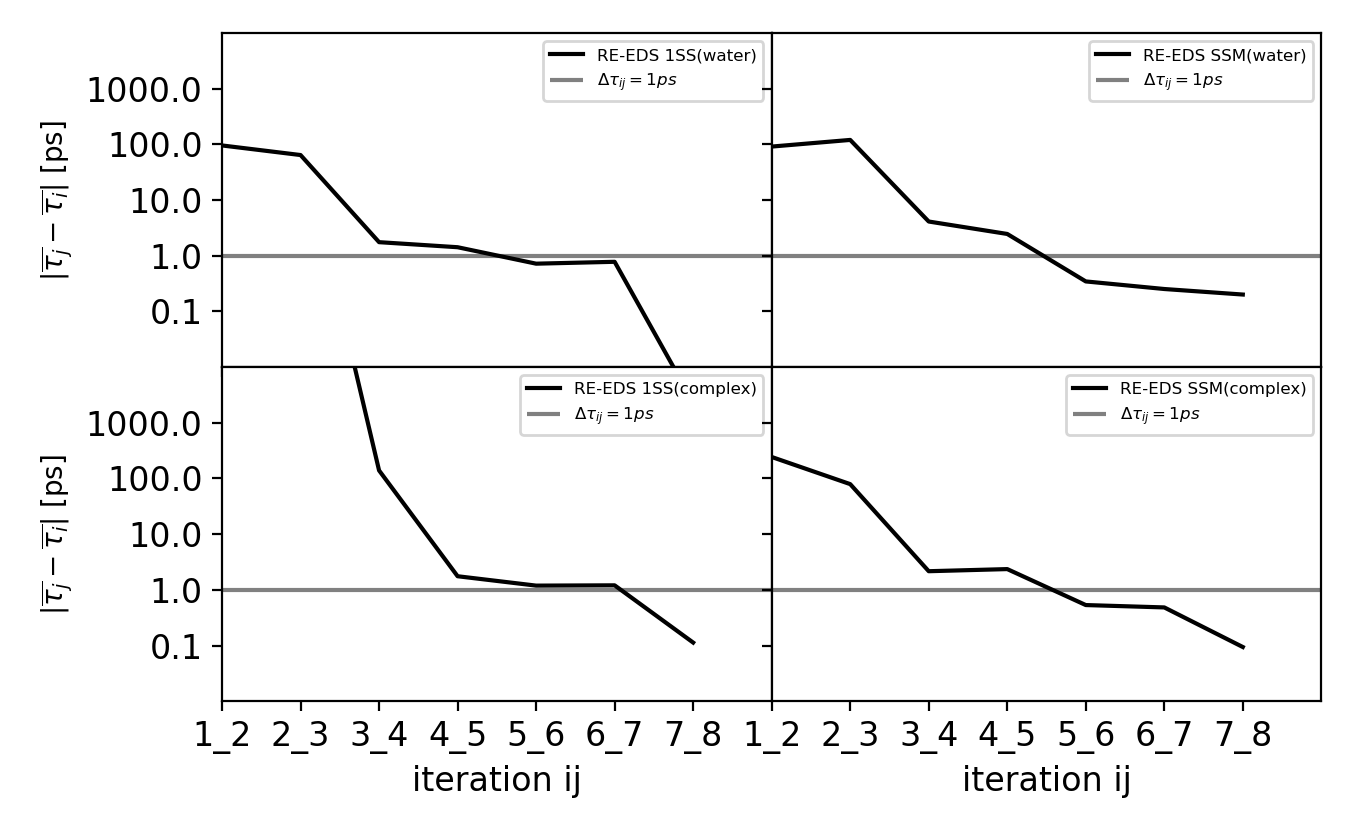
\includegraphics[width=\linewidth]{fig/results/ringOpening/paramOptimization/s_optimization_efficiency_RingOpening_log_scale.png}
\caption{Improvement of the average round-trip time between iterations $i$ and $j$ ($\overline{\tau}_j - \overline{\tau}_i$) on a logarithmic scale. An $s$-distribution was considered converged when ($\overline{\tau}_j - \overline{\tau}_i$) reached 1~ps.}
\label{SIfig:CHK1_RingOpening_soptimization_efficiency}
\end{figure}


\newpage

\section{Free-Energy Calculation}
\begin{table}[h]
\caption{Free-energy differences in water and in complex calculated from the production run of 4~ns of length with the RE-EDS 1SS and RE-EDS SSM approaches.}
\begin{center}
\begin{tabular}{ c c |c c |c c}
  \multicolumn{2}{c|}{Ligand} & \multicolumn{2}{c|}{RE-EDS 1SS} &\multicolumn{2}{c}{RE-EDS SSM}\\ 
  I & J  & water [kJ~mol$^{-1}$] & complex [kJ~mol$^{-1}$]  & water [kJ~mol$^{-1}$] & complex [kJ~mol$^{-1}$] \\
  \hline
        L17 &         L1 &       15.22 $\pm$ 0.15&       16.44 $\pm$ 0.22&  -13.61 $\pm$ 0.11&  16.63 $\pm$ 0.19\\
        L19 &         L1 &        6.73 $\pm$ 0.13&       -7.24 $\pm$ 0.16&   -1.95 $\pm$ 0.18&  -7.98 $\pm$ 0.19\\
        L20 &         L1 &      -48.59 $\pm$ 0.22&      -45.99 $\pm$ 0.21& -48.09 $\pm$ 0.13& -49.27 $\pm$ 0.35\\
        L21 &         L1 &      -67.83 $\pm$ 0.326&     -69.48 $\pm$ 0.20& -69.48 $\pm$ 0.16& -72.60 $\pm$ 0.85\\
        L19 &         L17 &      -8.49 $\pm$ 0.12&      -23.68 $\pm$ 0.25& -15.56 $\pm$ 0.18& -24.60 $\pm$ 0.13\\
        L20 &         L17 &     -63.81 $\pm$ 0.22&      -62.42 $\pm$ 0.19& -61.69 $\pm$ 0.14&  65.89 $\pm$ 0.33\\
        L21 &         L17 &     -83.05 $\pm$ 0.31&      -85.92 $\pm$ 0.29& -83.09 $\pm$ 0.17& -89.22 $\pm$ 0.84\\
        L20 &         L19 &     -55.32 $\pm$ 0.21&       38.75 $\pm$ 0.33& -46.13 $\pm$ 0.20& -41.29 $\pm$ 0.32\\
        L21 &         L19 &     -74.56 $\pm$ 0.31&      -62.24 $\pm$ 0.29& -67.52 $\pm$ 0.21& -64.62 $\pm$ 0.84\\
        L21 &         L20 &     -19.24 $\pm$ 0.35&      -23.50 $\pm$ 0.31& -21.39 $\pm$ 0.18& -23.33 $\pm$ 0.88\\
\end{tabular}
\end{center}
\label{SItab: RE-EDS_FE_RingCycleOpening_dFs}
\end{table}


\begin{figure}[h]
\centering
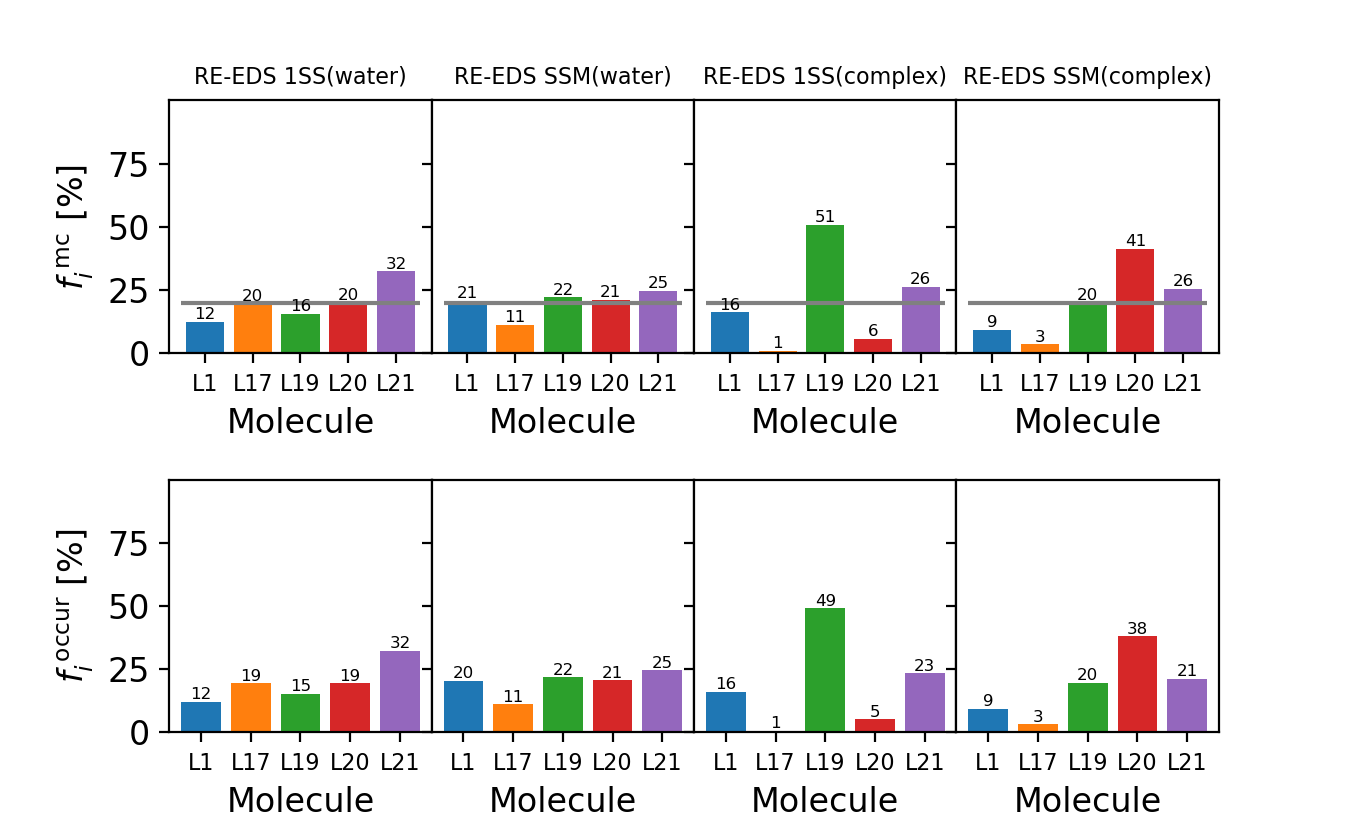
\includegraphics[width=\linewidth]{fig/results/ringOpening/FE/Reeds_RingOpening_production_sampling_s1.png}
\caption{Sampling of the end states in the final production run at replica $s=1.0$. Sampling was assessed by monitoring the dominant end state (top panels) and by counting all end states a potential energy below $T_{i}^{phys}$ (see Table \ref{SItab:RingCycleOpenin_PotentialTresholds}) (bottom panels). Ideally, the sampling fraction as dominating end state should be 1/$N$ (Eq. (8) in the main text) for all end states, indicated as a black horizontal line.}
\label{SIfig:CHK1_RingOpening_soptimization_final_Sampling_s1}
\end{figure}

\begin{figure}[h]
\centering
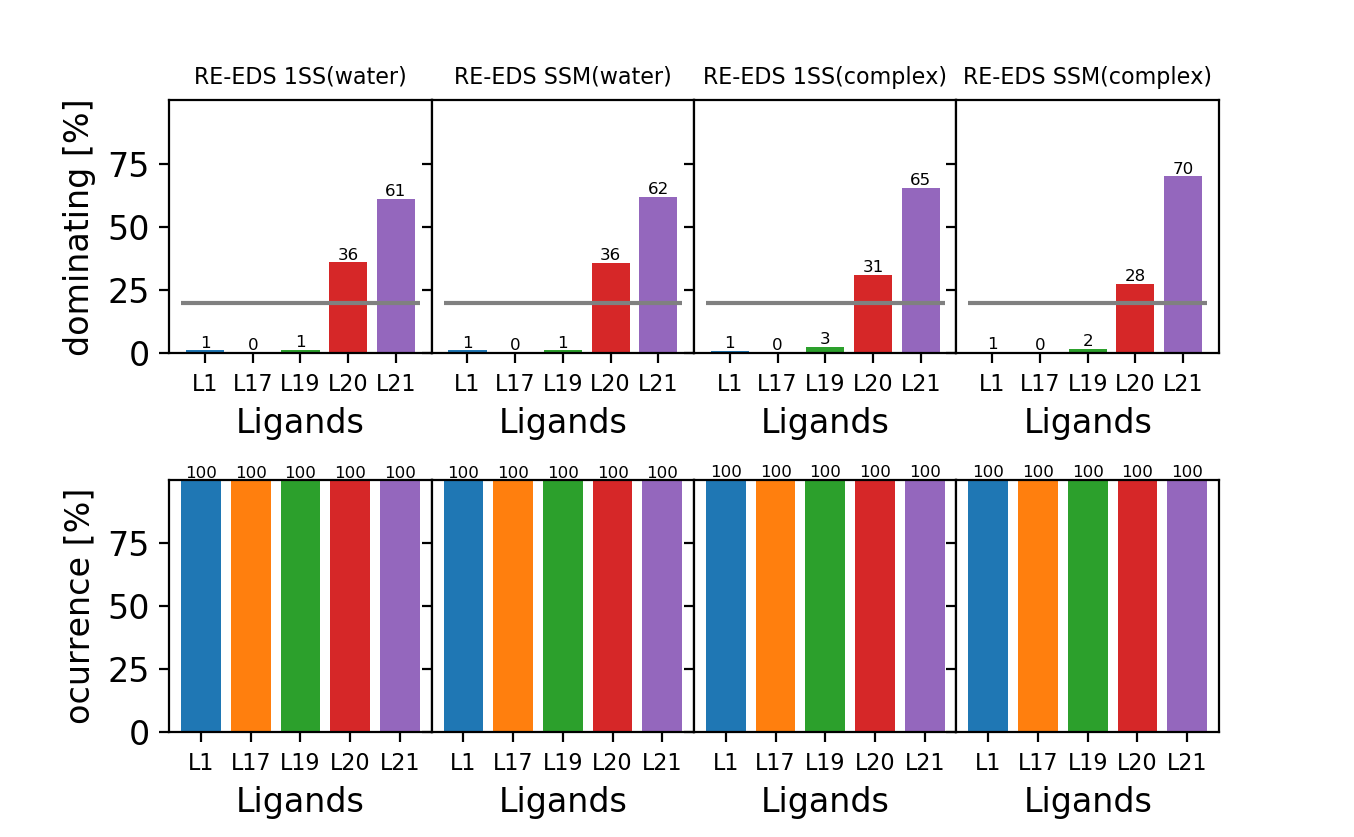
\includegraphics[width=\linewidth]{fig/results/ringOpening/FE/Reeds_RingOpening_production_sampling_underS.png}
\caption{Sampling of the end states in the final production run at the undersampling replica position $s=0.0032$. Sampling was assessed by monitoring the dominant end state (top panels) and by counting all end states a potential energy below $T_{i}^{phys}$ (see Table \ref{SItab:RingCycleOpenin_PotentialTresholds}) (bottom panels). Ideally, the sampling fraction as dominating end state should be 1/$N$ (Eq. (8) in the main text) for all end states, indicated as a black horizontal line.}
\label{SIfig:CHK1_RingOpening_soptimization_final_Sampling_undersampling}
\end{figure}

\begin{figure}[h]
\centering
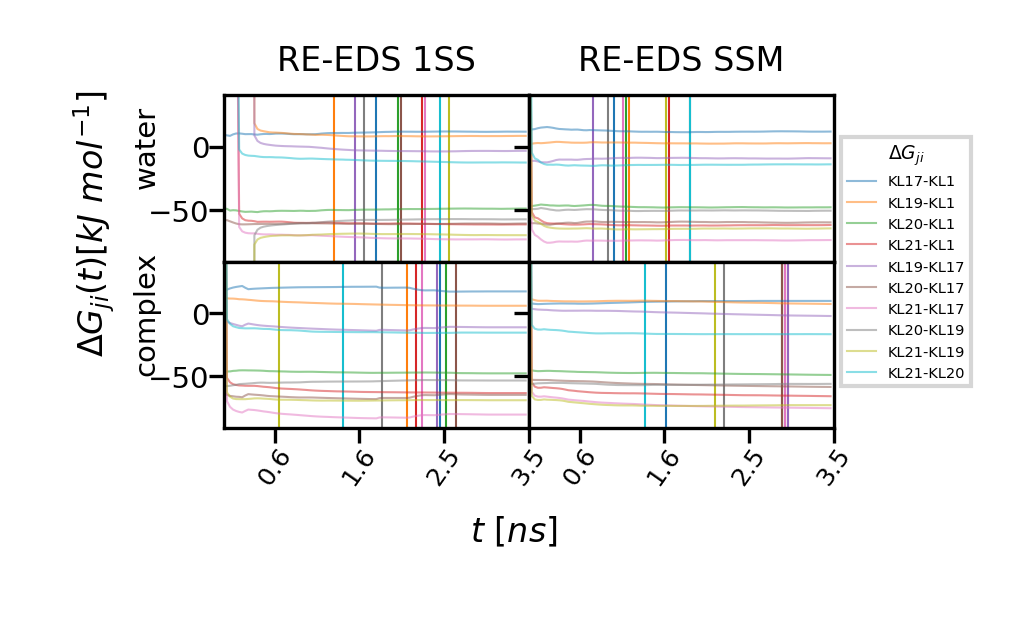
\includegraphics[width=\linewidth]{fig/results/ringOpening/FE/dF_RingOpening_Convergence.png}
\caption{Convergence analysis of the RE-EDS production runs (total 4~ns): Free-energy differences relative to the final free-energy results after 4~ns are plotted as a function of the simulation time. The vertical lines indicate when a particular $\Delta G_{ji}$ value was found to be converged (deviation below 0.25~kJ~mol$^{-1}$).}
\label{SIfig:CHK1_RingOpening_dF_convergence}
\end{figure}

%\bibliography{manual_ref.bib}

 